\chapter{Messbrücken und Messverstärker}
\begin{table}[h]
	\centering
	\begin{tabular}{|c|c|}
		\hline 
		Teilübung 	& Messbrücken und Messverstärker \\
		\hline 
		Teilübungsnr. 		& 2	 \\ 
		\hline 
		Datum 		& 29.11.2018 \\ 
		\hline 
		Messplatzbez. 	& CA0406-6  \\
		\hline
	\end{tabular} 
	\caption{Grundlegende Information der 3. Laborübung}
\end{table}
\noindent
\begin{table}[h]
	\begin{tabular}{|c|c|}
	\hline 
	Gerät & Bezeichnung \\ 
	\hline 
	Spannungsquelle & Rigol DP832\\ 
	\hline 
	Spannungsquelle für Heizelement & Konstanter T1 K 30 B 0,8 \\ 
	\hline 
	Kapazitätsdekade & Danbridge DK45\\ 
	\hline 
	Widerstandsdekaden & Goerz \\ 
	\hline 
	Temperaturmessung & Mastech MS8221C\\ 
	\hline 
	Funktionsgenerator & Siglent SDG1025\\ 
	\hline 
	Digitales Speicheroszilloskop & Agilent DSO-X 2002A\\ 
	\hline 
	\end{tabular} 
	\centering
	\caption{Verwendete Messgeräte}
	\label{tb:messgeraete}
\end{table}

\subsubsection{Eigentumsbestätigung}
Hermit bestätigen die Studierenden der Gruppe 20, alle Messungen selbst durchgeführt und für die Berechnungen ausschließlich diese Messergebnisse herangezogen zu haben. \\ \\
\begin{tabular*}{\textwidth}{c|c|c}
	Patrick Mayr & Katharina Kralicek & Oskar Fürnhammer \\ 
	01526681 & 01611844 & 01329133 \\ 
\end{tabular*}
%\begin{figure}
%	\includegraphics[width=\textwidht]{./img/ch3/}
%\end{figure}
\section{Wheatstone-Abgleich-Messbrücke}
\subsection{DC-Messbrücke}
Um den parasitären Widerstand eines realen Kondensators messen zu können, wurde eine DC-Messbrücke nach dem Modell in Abb. \ref{fig:dc_messbruecke} aufgebaut. 
\begin{figure}[H]
	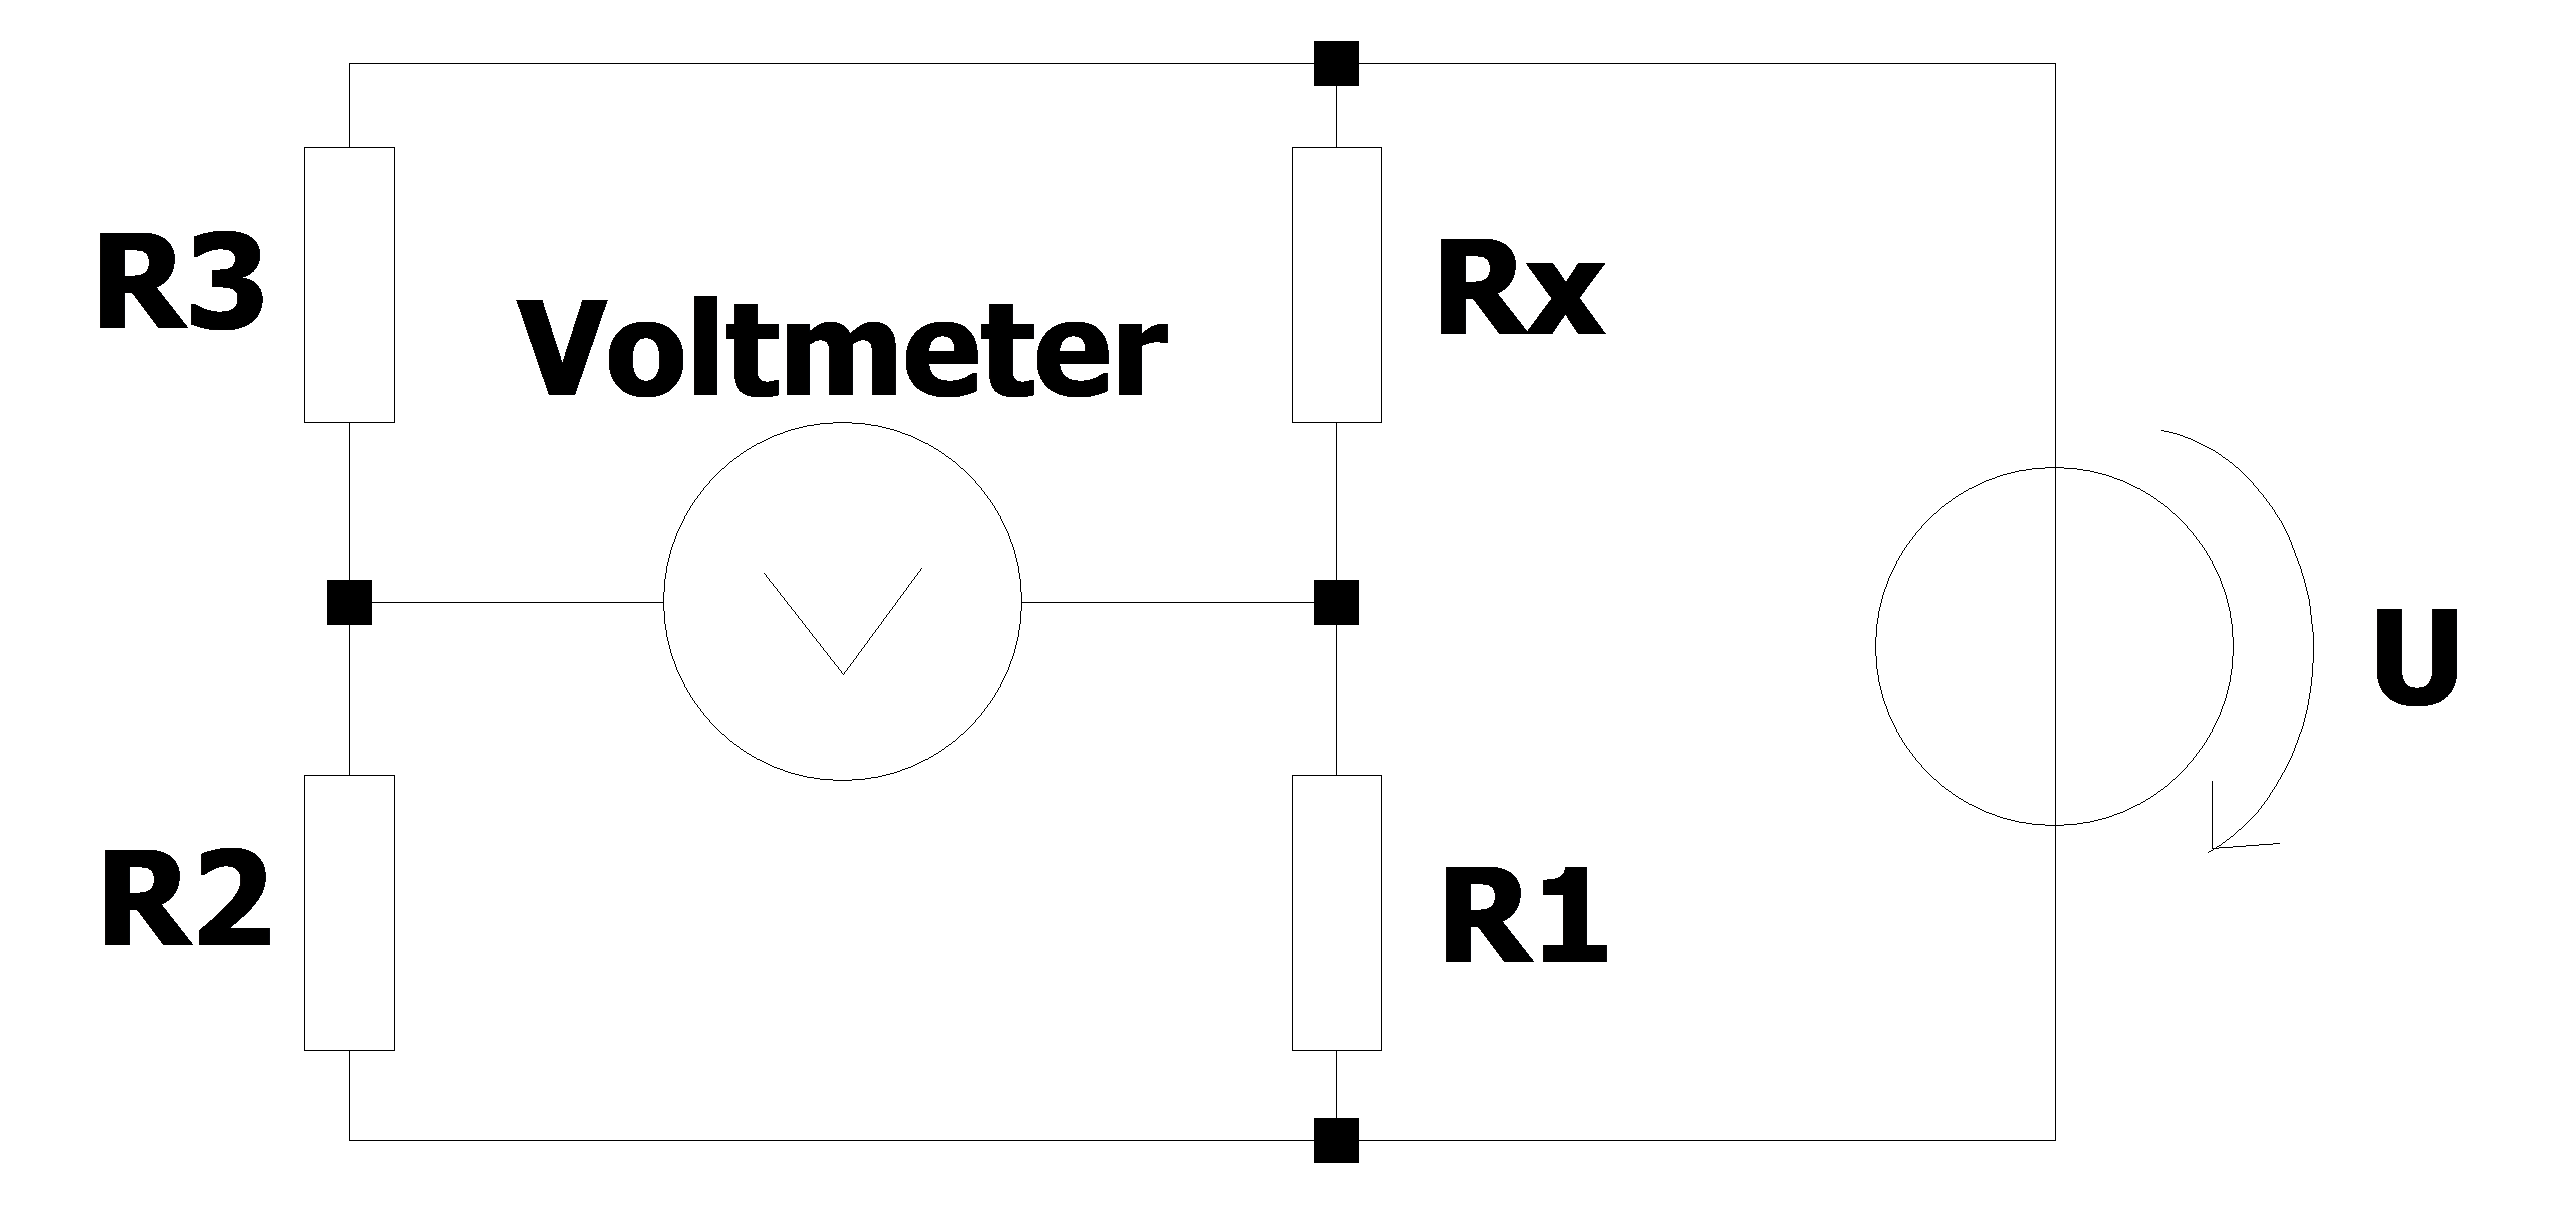
\includegraphics[width=\textwidth]{./img/ch3/DC_Wheatstone_Messbruecke.png}
	\label{fig:dc_messbruecke}
	\caption{DC Messbrücke}
\end{figure}
Für die Widerstände $R_1$ bis $R_3$ wurden Widerstandsdekaden verwendet, deren eingestellte Werte in Tabelle \ref{tb:dc_bt} nachzulesen sind. Der parasitäre Widerstand errechnet sich durch die Abgleichbedingung 
\begin{equation}
	R_1 R_3 = R_2 R_x
\end{equation}
zu 
\begin{equation}
	R_x=\frac{R_1 R_3}{R_2} = 6.86\,\text{M}\Omega\,.
\end{equation}
\begin{table}[h]
	\begin{tabular}{|c|c|}
	\hline 
	Bauteilbezeichnung & Wert [k$\Omega$] \\ 
	\hline 
	$R_1$ & 110 \\ 
	\hline 
	$R_2$ & 160.4 \\ 
	\hline 
	$R_3$ & 10 \\ 
	\hline 
	\end{tabular}
	\centering
	\label{tb:dc_bt}
	\caption{•}
\end{table}
Ist die Brücke nicht abgeglichen, so stellt sich eine Differenzspannung $U_d$ ein, die wiederum linear von der Versorgungsspannung abhängt, gemäß der Formel 
\begin{equation}
	U_d = U \frac{R_1 R_3-R_2 R_x}{R_x+R_1)(R_2+R_3)} = k U.
\end{equation}
Dies ist auch relevant für die Wahl einer geeigneten Versorgungsspannung, denn die Messbereiche der Multimeter sind sowohl nach unten, als auch nach oben begrenzt. Wird nun die Versorgungsspannung zu niedrig gewählt, so kann es passieren, dass die Brücke nicht vollständig abgeglichen ist, das Multimeter jedoch trotzdem keine Spannung anzeigt. Deswegen ist die Versorgungsspannung jedenfalls maximal zu wählen. Bei der vorliegenden Messung wurden daher $30\,$V gewählt, die Maximalspannung der Spannungsquelle. \\
Für die Messung an der vorliegenden Schaltung kann sowohl ein Voltmeter, als auch ein Amperemeter verwendet werden, da der Innenwiderstand des Multimeters keinen Einfluss auf die Schaltung hat. Dies ergibt sich daraus, dass für eine abgeglichene Brücke kein Strom über das Multimeter fließt.

\subsection{AC-Messbrücke}
Nun soll die Kapazität des realen Kondensators gemessen werden, was mithilfe der AC-Messbrücke, in Abb. \ref{fig:ac_messbruecke} zu sehen, möglich ist. 
\begin{figure}[H]
	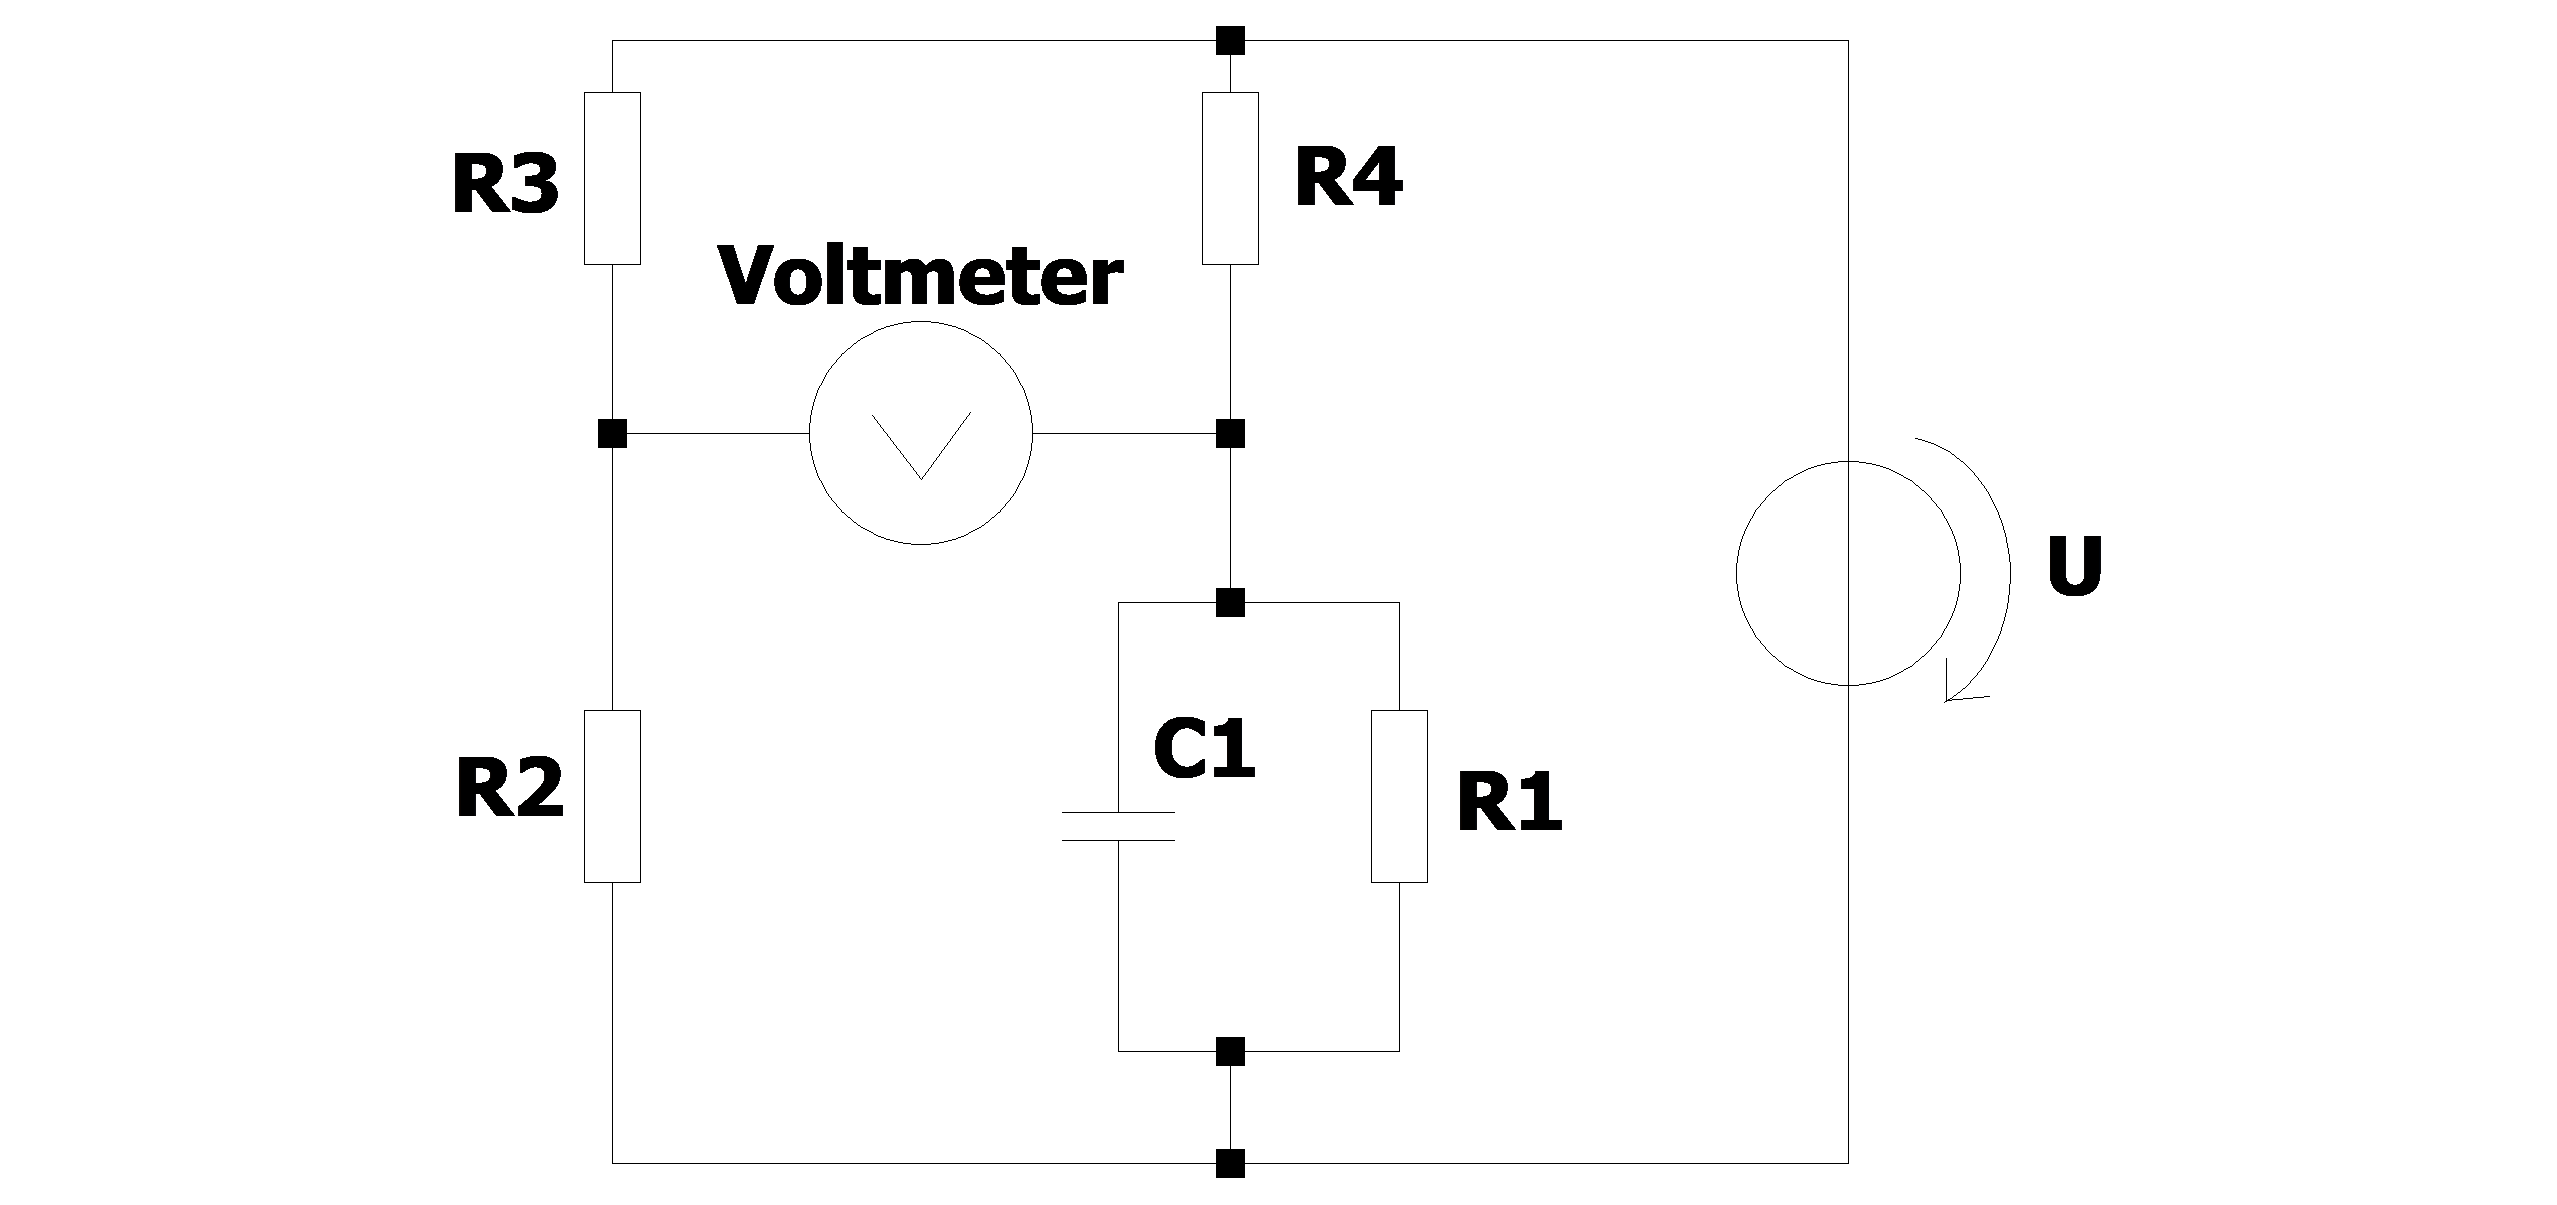
\includegraphics[width=\textwidth]{./img/ch3/AC_Wheatstone_Messbruecke.png}
	\label{fig:ac_messbruecke}
	\caption{X}
\end{figure}
Die Werte der Widerstandsdekaden und der nun hinzugefügten Kapazitätsdekade sind in Tabelle \ref{tb:ac_bt} abzulesen. Als Versorgungsspannung wurde diesmal eine Sinusspannung mit einer Amplitude von 10V und einer Frequenz von 1kHz gewählt, eingespeist durch den Signalgenerator des Oszilloskops. Die für den Abgleich dieser Messbrücke zu beachtenden Bedingungen sind
\begin{equation}
	Z_1 Z_3 = Z_2 Z_x\,
\end{equation}
oder in Realteilund Imaginärteil aufgespalten, 
\begin{align*}
	R_1 R_3 &= R_2 R_x \\ 
 	R_3 X_1 &= R_2 X_x 
\end{align*}
wobei $X_x$ die gesuchte Kapazität darstellt.
\begin{table}[h]
	\begin{tabular}{|c|c|}
	\hline 
	Bauteilbezeichnung & Wert [k$\Omega$] \\ 
	\hline 
	$R_1$ & 50k$\Omega$ \\ 
	\hline 
	$R_2$ & 3k$\Omega$ \\ 
	\hline 
	$R_3$ & 11.1k$\Omega$ \\ 
	\hline 
	$C$ & 3.8$\mu$F \\ 
	\hline 
	\end{tabular}
	\centering
	\label{tb:ac_bt}
	\caption{•}
\end{table}
Bei dieser Messung ist es uns jedoch nicht gelungen, die Brücke vollständig abzugleichen. Mit den in Tabelle \ref{tb:ac_bt} gelisteten Werten für die Dekaden blieb eine Differenzspannung $U_d$ von 22mV. In diesem Fall errechnet sich die gesuchte Kapazität zu
\begin{equation}
	X_x = \frac{R_3 X_1}{R_2} = 14.26\, \mu\text{F}.
\end{equation} 
%%	\begin{tabular}{|c|c|}
%%	\hline 
%%	Bauteilbezeichnung & Wert [k$\Omega$] \\ 
%%	\hline 
%%	$R_1$ & 50k$\Omega$ \\ 
%%	\hline 
%%	$R_2$ & 3k$\Omega$\\ 
%%	\hline 
%	$R_3$ & 11.1k$\Omega$\\ 
%	\hline 
%	$C$ & 3.8$\mu$F \\ 
%	\hline 
%	\end{tabular}
%	\centering
%	\label{tb:ac_bt}
%	\caption{•}
%\end{table}

\section{Messverstärker}
\subsection{Subtrahierverstärker}
\label{sec:subtrahier}
Es sollen durch diese Messungen sämtliche Eigenschaften eines Subtrahierverstärkers in einer Halbbrücke bestimmt werden. Dazu mussten zu Beginn alle Widerstände gewählt werden, wobei für eine angenommene Gegentaktverstärkung von $V=1200$ die Widerstände $R_1=R_3=100\Omega$ und $R_2=R_4=120k\Omega$ gewählt. \\
Für die Messung der Gegentaktverstärkung wird zwischen den beiden Eingängen ein zu verstärkendes Signal angelegt. Bei einem Eingangssignal der Frequenz $f=1\,$kHz und dem Spitze-Spitze-Spannungswert $u_e=4\,$mVpp wurde am Ausgang ein Spitze-Spitze-Spannugnswert von ua=3,7Vpp mit dem Oszilloskop gemessen. Daraus ergibt sich mit der Formel $V_\text{gemessen}=\frac{u_a}{u_e}=925$ die gemessene Gegentaktverstärkung. Da die absolute Abweichung der aus den Messwerten berechneten Verstärkung zur angenommenen Verstärkung doch 275 beträgt, ist es durchaus möglich, dass die angenommene Verstärkung zu hoch gesetzt war. Alternativ können Abweichungen auch durch Verluste in der Schaltung erklärt werden. \\
Nun wird der Eingangsoffset gemessen, indem bei Eingänge zusammen auf Masse gehängt werden, und anschließend am Oszilloskop bei DC Kopplung der DC RMS des Ausgangssignals abgelesen wird. Dabei ergab sich ein $U_a=420\,$mV, woraus mithilfe der Formel $U_e=\frac{U_a}{V}=0.35\,$mV der Eingangsoffset errechnet werden kann. Der Eingangsoffset eines OPVs wird durch seinen internen Aufbau hervorgerufen und tritt daher bei allen OPVs auf. \\
Um die Gleichtaktunterdrückung (Common Mode Rejection Ratio) zu ermitteln, legt man an beiden Eingängen das gleiche Signal an und betrachtet den Ausgang am Oszilloskop. Für eine Eingangsspannung von $u_e=12\,$Vpp und eine Frequenz von $f=100\,$Hz wurde am Ausgang $u_a=160\,$mVpp gemessen. Daraus ergibt sich mit der Formel
\begin{equation}
	A=\frac{u_a}{u_e}=\num{13.33e-3}
\end{equation}
die Gleichtaktverstärkung. Mit Formel 
\begin{equation}
	CMRR=20*log(\frac{V_gemessen}{A})=96.83\,\text{dB} 
\end{equation}
kommt man auf die Gleichtaktunterdrückung. \\
Um den RMS Wert des Rauschens zu messen, wurden die beiden Eingänge kurzgeschlossen und das Ausgangssignal mit dem Oszilloskop gemessen. Dabei ergab sich, mit eigestellter AC Kopplung, ein $U_a=1.8$mV, was dem Rauschen entspricht.

\subsection{Instrumentenverstärker}
Nun sollten die Merkmale eines Instrumentenverstärkers in einer Halbbrücke ermittelt werden. Der Widerstand RG wurde in dem Fall durch die angenommene Verstärkung $V=1000$ gemäß der Formel
\begin{equation}
	V=1+\frac{2R}{R_G}=1+\frac{50k\Omega}{R_G} 
\end{equation} auf $R_G=50\Omega$ festgelegt.
Sämtliche Messaufbauten erfolgen analog zu denen aus Unterpunkt \ref{sec:subtrahier} und werden aus diesem Grund hierbei etwas kürzer gefasst. \\
Aus der Messung für die Gegentaktverstärkung erhielt man ein $u_a=5.7\,$Vpp bei einem Eingang von $u_e=5$mVpp und einer Frequenz $f=100\,$Hz. Daraus errechnet sich V zu $\num{1,14e+3}$.\\
Der Eingangsoffset errechnet sich daher, mit einem gemessenen Ua=5mV zu $U_e=\frac{U_a}{V}=\num{4.39e-6}$. \\
Die Ausgangsspannung am Oszilloskop beträgt $u_a=30\,$mVpp, bei aufgebauter Schaltung für die Bestimmung der Gleichtaktunterdrückung und einem Eingang von $5\,$Vpp bei $f=100\,$Hz. Daraus ergibt sich ein $A=\num{6e-3}$, woraus eine CMRR von $105.58\,$dB folgt. \\
Für den Instrumentenverstärker wurde ein RMS Rauschen von $4.17$mV gemessen. \\
Zum Vergleich der beiden Verstärker sind in Tabelle \ref{tb:eigenschaften} nochmals alle Eigenschaften aufgelistet. Dabei erkennt man, dass der Instrumentenverstärker eine höher Gegentaktverstärkung, sowie einen geringeren Eingangsoffset und einen höheren CMRR hat. Hingegen hat der Subtrahierverstärker ein geringeres Rauschen.
\begin{table}
	\begin{tabular}{|c|c|c|}
	\hline 
	Eigenschaft & Subtrahierverstärker & Instrumentenverstärker \\ 
	\hline 
	Gegentaktverstärkung & 925 & $\num{1.14e+3}$ \\ 
	\hline 
	Eingangsoffset & 350 $\mu$V & 4.39 $\mu$V \\ 
	\hline 
	CMRR & 96.83 dB & 105.58 dB \\ 
	\hline 
	Rauschen & $1.8\,$mV & $4.17\,$mV \\ 
	\hline 
	\end{tabular}
	\centering
	\caption{•}
	\label{tb:eigenschaften}
\end{table}

\section{Ausschlag Messbrücke}
\subsection{Gewichtsmessung mit einer Halbbrücke}
Ein Dehnmessstreifen soll, in einer Halbbrückenschaltung verbaut, auf seine Funktionsweise getestet werden, wobei auch zusätzlich der Instrumentenverstärker aus Übung \ref{} angeschlossen wird. Konkret wird dabei mithilfe von Referenzgewichten der Spannungssausschlag bei Belastung der Messbrücke mit den Gewichten gemessen. \\
Bei 25 C wurde der Widerstand des Dehnmessstreifen als $R_{1d}=119.9\,\Omega$ gemessen, dementsprechend wurden die restlichen Widerstände gewählt.\\
Wie in Abb. \ref{fig:gewicht_mb} zu sehen, ist der Zusammenhang trotz Schwankungen annähernd linear. 
\begin{figure}[H]
	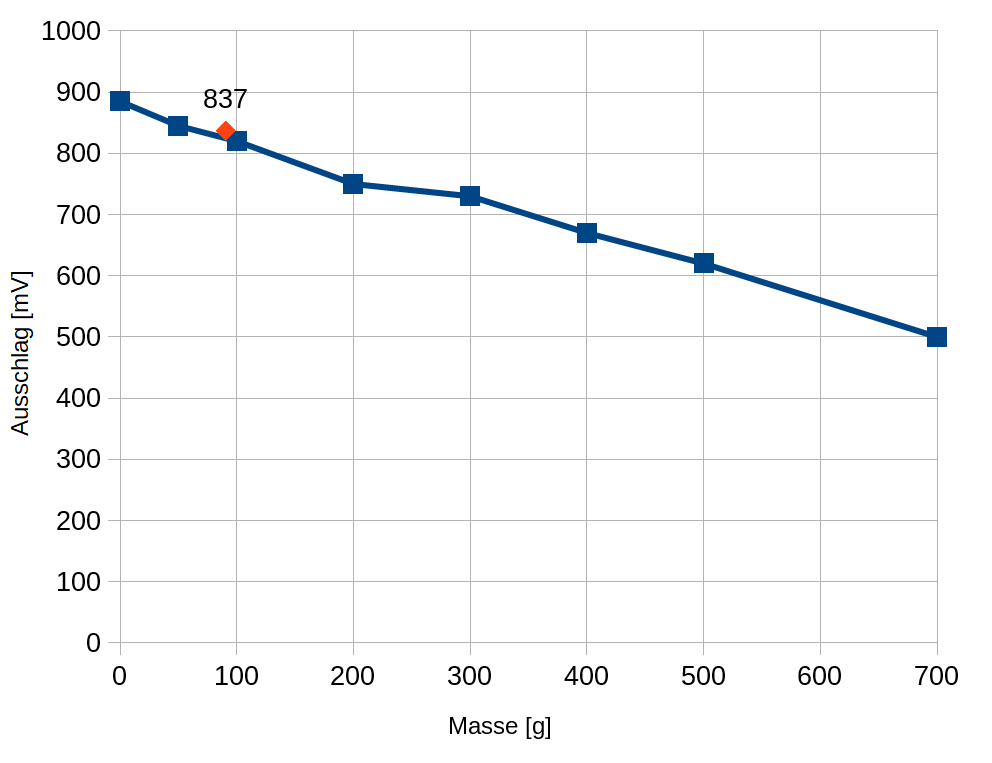
\includegraphics[width=\textwidth]{./img/ch3/GewichtsmessungHalbbruecke_3_3_1.png}
	\label{fig:gewicht_mb}
	\caption{X, HANDY!}
\end{figure}
Die Sensitivität der Schaltung wird dabei mithilfe der Formel
\begin{equation}
	 E(\Delta m) = \frac{U_2-U_1}{500g-0g}=\frac{620mV-885mV}{0,5kg-0kg}=-530mV/kg
\end{equation}
berechnet. \\
Der Offset am Ausgang des Messverstärkers entspricht der Spannung bei unbelastetem Dehnmessstreifen, also folglich $885\,$mV. Das lässt sich durch den Eingangsoffset des Instrumentenverstärkers erklären und dadurch, dass möglicherweise die Messbrücke nicht vollständig abgeglichen war, erklären. \\
Zusätzlich wurde das Gewicht eines IPhone SE durch die Schaltung bestimmt, mithilfe der Formel
\begin{equation}
	m=U_{gemessen}-\frac{U_{offset}}{E}=\frac{837mV-885mV}{-530m(V/kg)}=90\,g.
\end{equation}
Die Abweichung von den 113g, die der Hersteller für dieses Handy angegeben hat, lässt sich durch die niedrige Sensitivität der Messbrücke, sowie mögliche Störungen durch Stöße am Tisch erklären.

\subsection{Störeinflüsse einer Halbbrücken}
Um die möglichen Störeinflüsse durch die Temperaturabhängigkeit eine Halbbrücke einschätzen zu können, wurde nun ein Heizelement, gespeist durch einen Funktionsgenerator, benutzt, um sowohl die Verstärkerausgangsspannung, als auch das Rauschen bei verschiedenen Temperaturen aufzuzeichnen. Die Temperaturmessung erfolgte hierbei über ein geeignetes Multimeter, während das Rauschen sowie der Wert der Verstärkerausgangsspannung mit dem Oszilloskop bestimmt wurden. \\
Durch einen Fehler bei der Messung, der erst im Nachhinein aufgefallen ist, liegen für die Messung nicht ab der Starttemperatur des Heizelements von 25 C vor, sondern nur Werte ab einer Temperatur von 33  C. Die Werte für die Verstärkerausgangsspannung sind, wie man in Abb. \ref{fig:temp_mb} sehen kann, nicht sehr aussagekräftig, da sie zu stark schwanken, um einen funktionalen Zusammenhang erkennen zu können. Das Rauschen hingegen bleibt verhältnismäßig konstant über die Temperatur.
\begin{figure}[H]
	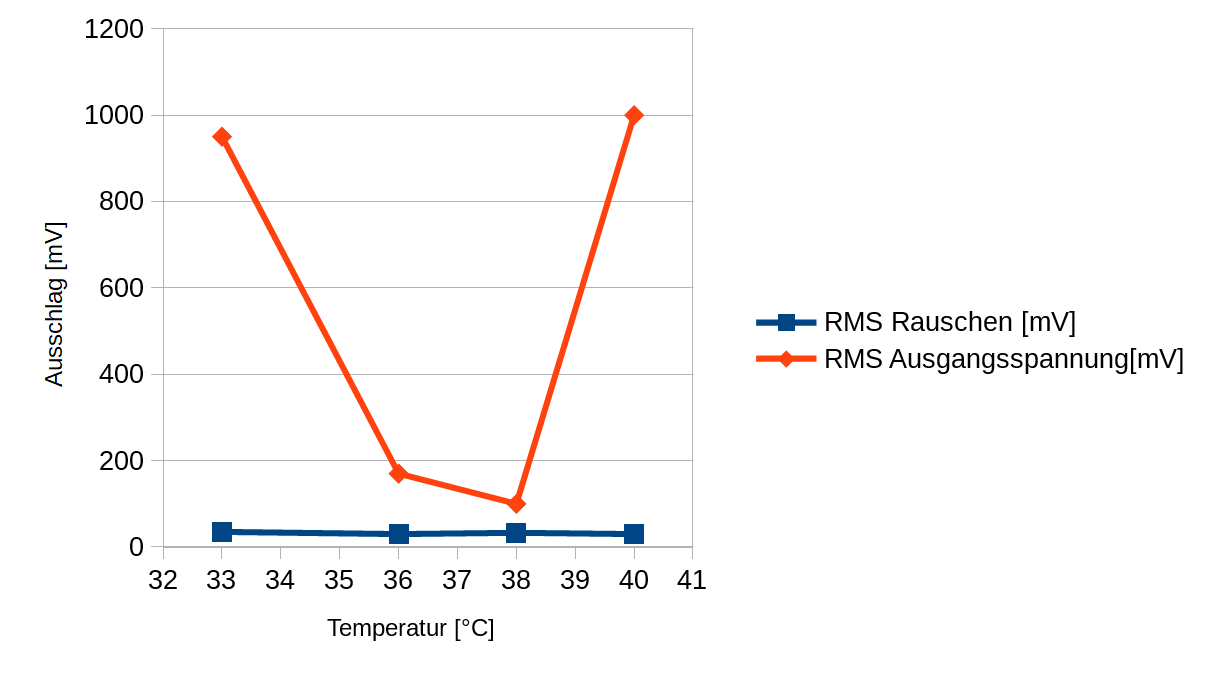
\includegraphics[width=\textwidth]{./img/ch3/TemperaturmessungHalbbruecke_3_3_2.png}
	\label{fig:temp_mb}
	\caption{X}
\end{figure}

\subsection{Vollbrücke}
Nun wird die Halbbrücke zur Vollbrücke erweitert, und sämtliche zuvor durchgeführte Messungen werden wiederholt, um eine Vergleich zwischen beiden Schaltungen ziehen zu können. Die Messung wurde bei 27 C gemacht, da nicht auf vollständiges Abkühlen des Heizelements gewartet werden konnte. 
\begin{figure}[H]
	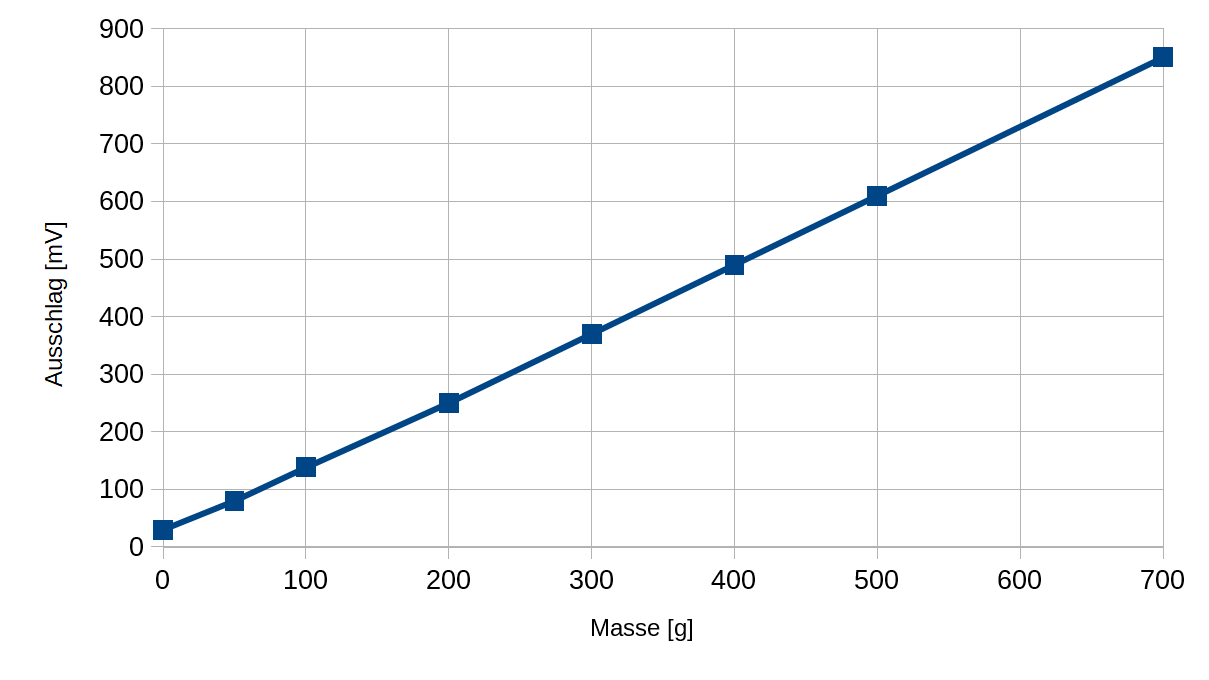
\includegraphics[width=\textwidth]{./img/ch3/GewichtsmessungVollbruecke_3_3_3.png}
	\label{fig:gewicht_vb}
	\caption{X}
\end{figure}
In Abb. \ref{fig:gewicht_vb} sind die einzelnen Ausschläge für verschiedene Gewichte dargestellt, und es ist ein nahezu linearer Zusammenhang erkennbar, mit kaum Abweichungen. Die Sensitivität errechnet sich, wie schon zuvor, aus 
\begin{equation}
	E(\Delta m)=\frac{U_2-U_1}{500g-0g}=1.16\,V/kg,
\end{equation}
was betragsmäßig um circa einen Faktor 2 größer ist als die Sensitivität einer Halbbrücke. \\
Auch für Vollbrückenschaltung wurde nun durch das Heizelement die Temperatur des Dehnmessstreifen erhöht und die Verstärkerausgangsspannung sowie das Rauschen der Schaltung aufgenommen. 
\begin{figure}[H]
	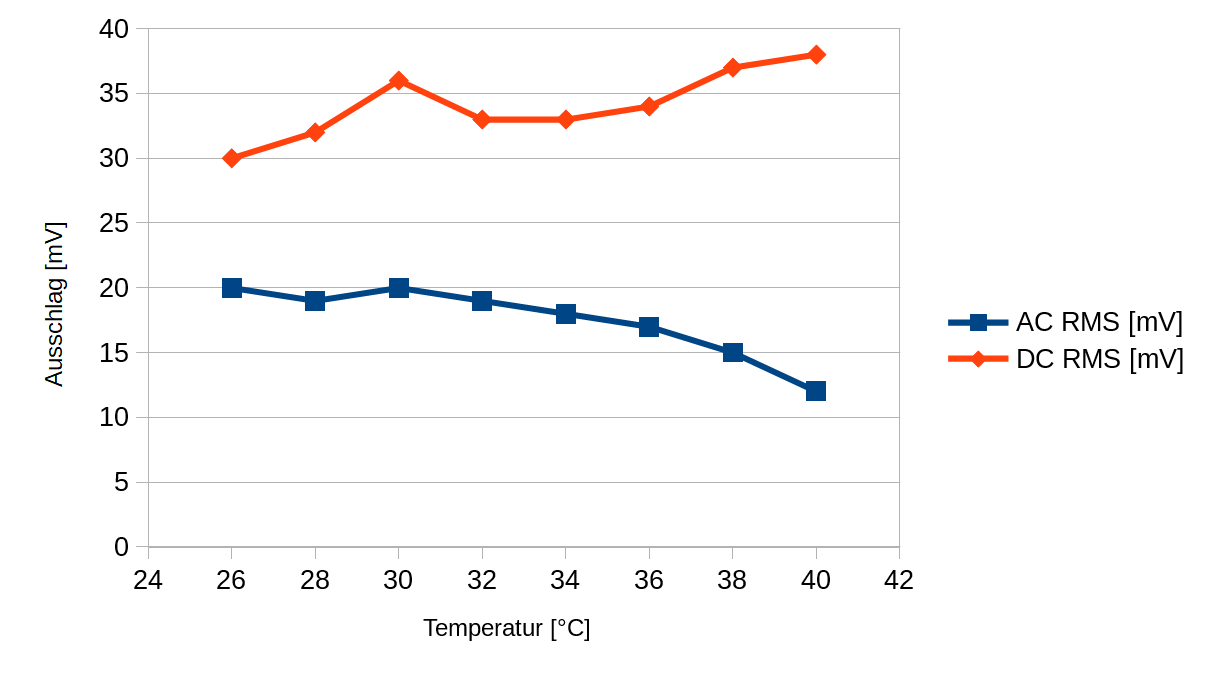
\includegraphics[width=\textwidth]{./img/ch3/TemperaturmessungVollbruecke_3_3_3.png}
	\label{fig:temp_vb}
	\caption{X}
\end{figure} \noindent
In Abb. \ref{fig:temp_vb} kann man sehr schön sehen, dass mit steigender Temperatur auch die Ausgangsspannung eine leichte Steigung aufweist, mit einem Ausreißer nach oben bei 36 C. Das Rauschen ist auf jeden Fall geringer als bei der Halbbrücke, wobei man jedoch erkennen kann, dass mit steigender Temperatur das Rauschen stärker sinkt, entgegen jeder physikalischen Erwartung. Somit ist dies vermutlich eher auf einen Messfehler zurückzuführen, als auf eine tatsächliche Auswirkung der Temperaturerhöhung.

\subsection{Tiefpassfilter zur Rauschreduzierung}
Um nun das Rauschen der Schaltung zu reduzieren, soll ein Tiefpassfilter, aufgebaut als RC-Glied, nun hinzugeschalten werden. Für eine Kapazität von $10\,$nF und eine gewählte Grenzfrequenz von $100\,$Hz ergibt sich daher ein Widerstand von $159k\Omega$, wofür ein Widerstand von $150k\Omega$ in die Schaltung eingebaut wurde. Über die Formel $f=\frac{1}{2\pi R C}$ ergibt sich damit eine reale Grenzfrequenz von $106.1\,$Hz. \\
Die Messung des Rauschens am Oszilloskop ergab ohne den Filter $20\,$mV und mit hinzugeschaltetem Filter $1.6\,$mV, womit man eindeutig die Reduzierung des Rauschens sehen kann. Das Rauschen setzt sich in diesem Fall aus dem thermischen Rauschen, dem Rauschen der Schaltung, sowie Störung durch elektrische oder magnetische Felder zusammen.
